\documentclass{bredelebeamer}
\usepackage{subfig}

%%%%%%%%%%%%%%%%%%%%%%%%%%%%%%%%%%%%%%%%%%%%%%%%
\title[Kubernetes]{Kubernetes}
% Titre du diaporama

\subtitle{manage application, not machines}
% Sous-titre optionnel

\author{N. Salleron B. Affes}
% La commande \inst{...} Permet d'afficher l' affiliation de l'intervenant.
% Si il y a plusieurs intervenants: Marcel Dupont\inst{1}, Roger Durand\inst{2}
% Il suffit alors d'ajouter un autre institut sur le modéle ci-dessous.

\date{Lundi 12 Février 2018}
% Optionnel. La date, généralement celle du jour de la conférence

\subject{NMV}
% C'est utilisé dans les métadonnes du PDF

\logo{

\includegraphics[scale=0.03]{images/logo.jpg}
}

%%%%%%%%%%%%%%%%%%%%%%%%%%%%%%%%%%%%%%%%%%%%%%%%%%%%%%%%%%%%%%%%%%%%%
\begin{document}

\begin{frame}
  \titlepage
\end{frame}

\begin{frame}{Sommaire}
  \tableofcontents
  % possibilité d'ajouter l'option [pausesections]
\end{frame}

\section{Introduction}
\subsection{Introduction}

\begin{frame}{Historique}
\begin{block}{Une longue émergence}
\begin{itemize}
\item Borg
	\begin{itemize}
	\item Démarrage en 2004.
	\item Développé en interne.
	\item Manager de containers.
	\item Objectif : réduction des coups en partageant machines et applications.
	\item \textbf{Non open-source.}
	\end{itemize}	\pause
\item Omega	
	\begin{itemize}
	\item Fils de Borg.
	\item Amélioration de l'écosystème apporté par Borg.
	\item  \textbf{Non open-source.}
	\end{itemize}   \pause
\item Kubernetes
	\begin{itemize}
	\item Adaptable à plusieurs infrastructure cloud.
	\item  \textbf{Open-source.}
	\end{itemize}
\end{itemize}
\end{block}
\end{frame}

\begin{frame}{Introduction}
%Texte normal \alert{Texte Alert}  \exemple{Texte exemple} \emph{Texte emphase}
\begin{columns}
\begin{column}{0.5\textwidth}

Nom venant du Grec, crée par 3 ingénieurs de chez Google en 2014.
\begin{itemize}
\item \textit{Orchestrateur} - Gestionnaire de conteneur.
\item Exécute et manages des containers.
\item Propose une API permettant la gestion de plusieurs clouds (Google, Microsoft, Amazon, et pleins d'autres).
\item 100\% Open Source écrit en Go.
\end{itemize}
\vspace{10px}
Il permet de se focus sur les applications et non sur le déploiement.  \\
Google exécute 2 milliards de conteneurs par semaine avec ces systèmes.\\
Dernière version : 1.9.3 (sorti il y a 3 jours) \\ 

\vspace{10px}
\textit{"manage application, not machines" - Tim Hockin}

\end{column}
\begin{column}{0.5\textwidth}
\begin{figure}
\centering

\includegraphics[scale=0.15]{images/img1.png}
\caption{Logo de Kubernetes}
\end{figure}
\end{column}
\end{columns}
\end{frame}

\begin{frame}{Popularité}
Évolution des recherches entre \textcolor{Framableu}{Kubernetes}, \textcolor{Framarouge}{Mesos}, \textcolor{Framajaune}{Docker Swarm}
\begin{center}
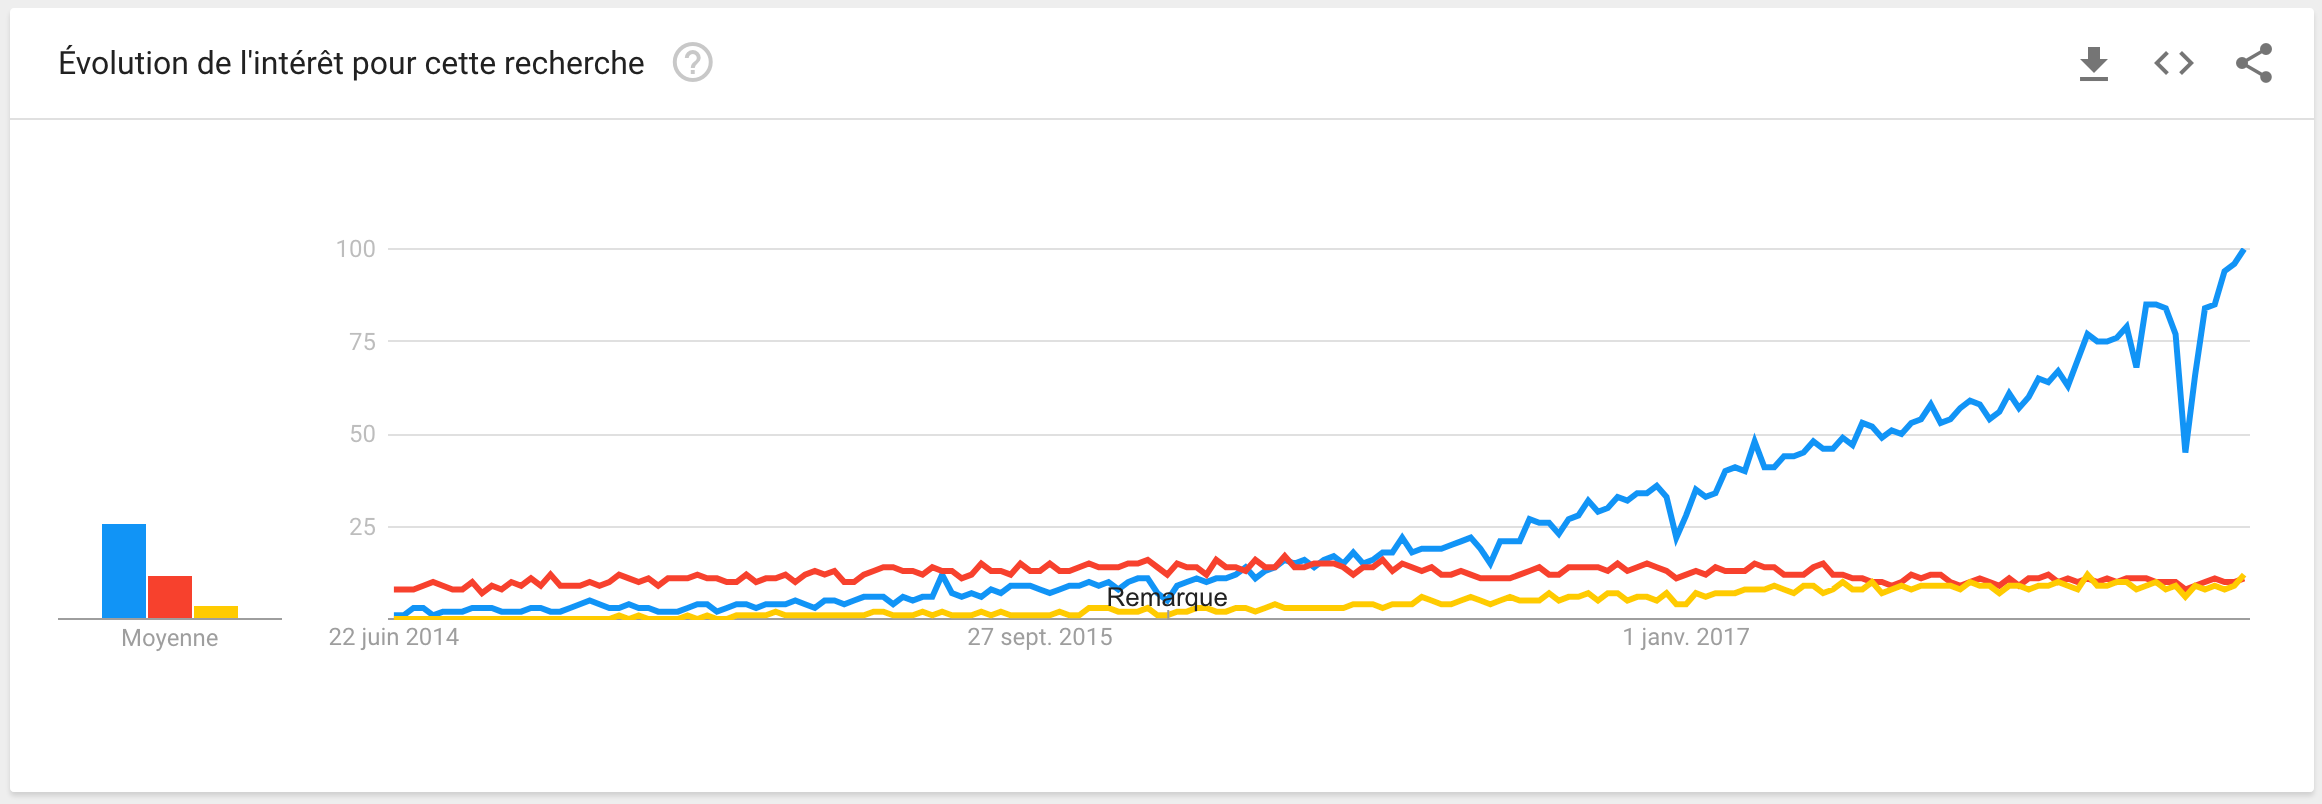
\includegraphics[scale=0.25]{images/img2.png}
\end{center}\pause
Une communauté très active : 
\begin{itemize}
\item Actuellement 61000 commits avec plus de 1500 contributeurs
\end{itemize}
\begin{center}
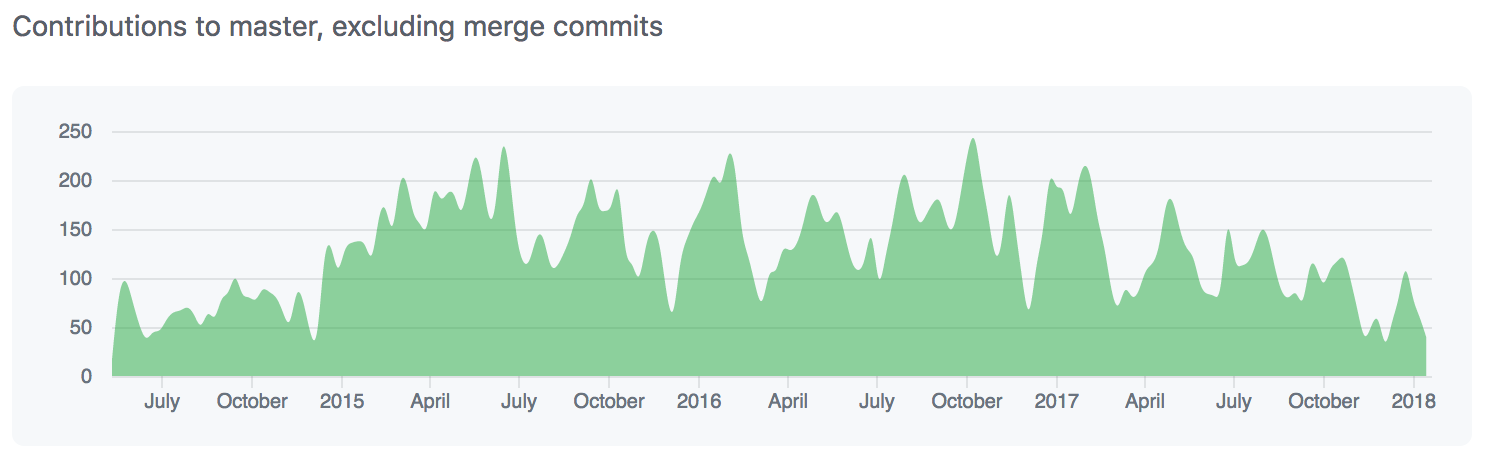
\includegraphics[scale=0.3]{images/img3.png}
\end{center}
\end{frame}






\end{document}




